%----------------------------------------------------------------------------------------
% Packages and other document configurations
%----------------------------------------------------------------------------------------

\documentclass[
    swedish, english,                % english main language
%    english,swedish,                % swedish main language
]{LnuCmThesis}

\usepackage{settings}

\addbibresource{example.bib}
%\addbibresource{example2.bib} % Additional bib file.

%\watermark % DRAFT is the default watermark text
%\watermark[UTKAST]

%----------------------------------------------------------------------------------------
% Thesis information
%----------------------------------------------------------------------------------------

%\title{}      % Your Title/Din titel
%\subtitle{}   % Your Subtitle/Din undertitel
%\author{}     % Your Name/Ditt namn
%\supervisor{} % Your Supervisor/Din handledare

\begin{document}

\frontmatter{} % Use roman page numbering style (i, ii, iii, iv...) for the front matters pages

%----------------------------------------------------------------------------------------
% Title page
%----------------------------------------------------------------------------------------

\maketitle

%----------------------------------------------------------------------------------------
% Abstract page
%----------------------------------------------------------------------------------------

\begin{abstract}
    \lipsum[1]

    \keywords{lorem\cite{loremlipsum}, ipsum, dolor, sit, amet, consectetuer, adipiscing, elit}
\end{abstract}

% Abstract in secondary language
\begin{abstract}[swedish] %[english] 
    Träutensilierna i ett tryckeri äro ingalunda en faktor där trevnadens ordningens och ekonomiens upprätthållande, och dock är det icke sällan som sorgliga erfarenheter göras ordningens och ekon och miens därmed upprätthållande. Träutensilierna i ett tryckeri äro ingalunda en oviktig faktor, för trevnadens ordningens och och dock är det icke sällan.

    \keywords{träutensilierna, tryckeri, äro, ingalunda, faktor, trevnadens, ordningens}
\end{abstract}

%----------------------------------------------------------------------------------------
% Acknowledgements page
%----------------------------------------------------------------------------------------

\begin{acknowledgements}
    \lipsum[1]
\end{acknowledgements}

%----------------------------------------------------------------------------------------
% Table of Contents and list of Figures/Tables/Listings pages
%----------------------------------------------------------------------------------------

\tableofcontents % Prints the main table of contents

\listoffigures % Prints the list of figures

\listoftables % Prints the list of tables

\lstlistoflistings{} % Prints the list of listings

%----------------------------------------------------------------------------------------
% Thesis content - Chapters
%----------------------------------------------------------------------------------------

\mainmatter{} % Use numeric page numbering style (1, 2, 3, 4...) for the content pages.

% Main chapter title
\chapter{Heading on Level 0 (chapter)}\label{chapter1} 

\lipsum[1]

%----------------------------------------------------------------------------------------
%	Heading on Level 1 (section)
%----------------------------------------------------------------------------------------

\section{Heading on Level 1 (section)}

\lipsum[2]

%-----------------------------------
%	Heading on Level 2 (subsection)
%-----------------------------------

\subsection{Heading on Level 2 (subsection)}

\lipsum[3]

%-----------------------------------
%	Heading on Level 3 (subsubsection)
%-----------------------------------

\subsubsection{Heading on Level 3 (subsubsection)}

\lipsum[4]

%-----------------------------------
%	Heading on Level 4 (paragraph)
%-----------------------------------

\paragraph{Heading on Level 4 (paragraph)}

\lipsum[5]

%----------------------------------------------------------------------------------------
%	Figures, Tables and Listings
%----------------------------------------------------------------------------------------

\section{Cite, Footnote, Figure, Table and Listings}

Lorem ipsum~\cite{loremlipsum} dolor sit amet, consectetuer adipiscing elit. Ut purus elit, vestibulumut, placerat ac, adipiscing vitae, felis. Curabitur dictum gravida mauris. 

\subsection{Figure}

The figure\ref{fig:appleblossom1} is a framed image of apples to be.

\begin{figure}[ht!]
    \frame{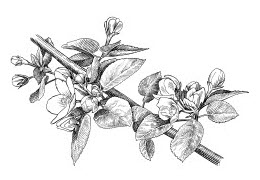
\includegraphics[width=0.7\linewidth]{images/lnu_apple_blossom.jpg}}
    \caption{Apple blossom.}\label{fig:appleblossom1}
\end{figure}

\subsection{Table}

The table\ref{table:simpletable} is a simple one.

\begin{table}[ht!]
    \begin{tabular}{ |c|c|c| } % chktex -2 (supress user regular expression warning)
        \hline                 % chktex -2 
        Col1 & Col2 & Col3 \\
        \hline                 % chktex -2 
        cell1 & cell2 & cell3 \\ 
        cell4 & cell5 & cell6 \\ 
        cell7 & cell8 & cell9 \\ 
        \hline                 % chktex -2 
    \end{tabular}
    \caption{A simple table.}\label{table:simpletable}
\end{table}

\subsection{Listings}

The listing\ref{lst:pythonhello} is a simple Python example.

\begin{lstlisting}[caption=Python example, label=lst:pythonhello, language=python]
# This is a comment
firstVariable = 'Hello World'
print(firstVariable.upper())
\end{lstlisting}

The listing\ref{lst:jshello} is a simple JavaScript\footnote{No official syntax highlighting is available for the JavaScript language.} example.

\begin{lstlisting}[caption=JavaScript example, label=lst:jshello]
// This is a comment
let firstVariable = 'Hello World'
console.log(firstVariable.toUpperCase())
\end{lstlisting}
%\include{chapters/chapter02}
%\include{chapters/chapter03}

%----------------------------------------------------------------------------------------
% References
%----------------------------------------------------------------------------------------

\printbibliography[heading=bibintoc]

%----------------------------------------------------------------------------------------
% Appendices
%----------------------------------------------------------------------------------------

\begin{appendices} % Switches the document from generating chapters to producing appendices.

    \chapter{Appendix Title Here}\label{appendixA}

\lipsum[60]
    %\input{appendices/AppendixB}
    %\input{appendices/AppendixC}

\end{appendices}

\backmatter{}
\end{document}